\documentclass[11pt]{article}
\usepackage[a4paper,margin=2.2cm]{geometry}
\usepackage{amsmath,amssymb}
\usepackage{booktabs}
\usepackage{enumitem}
\usepackage{xcolor}
\usepackage{tikz}
\usepackage{caption}
\usetikzlibrary{arrows.meta,positioning,fit,backgrounds}
\usepackage[hidelinks]{hyperref}
\newcommand{\code}[1]{\texttt{\small #1}}
\newcommand{\grd}{\textcolor{green!50!black}{\textbf{[grounded]}}}
\newcommand{\opn}{\textcolor{orange!80!black}{\textbf{[open]}}}
\tikzset{
  box/.style ={draw, rounded corners, align=center, font=\small, fill=blue!4, minimum height=8mm},
  hl/.style  ={draw, rounded corners, align=center, font=\small, fill=orange!12, very thick, minimum height=8mm},
  arr/.style ={-{Stealth[length=2.2mm]}, thick},
}
\title{\textbf{From the CR kernel to a spectral field basis}\\[2pt]
  \large Chebyshev filters, walks/cycles/Berge as spectral components, and an honest read on the
  ``Fourier field theory'' intuition}
\author{Dr.\ Csaba Hajdu}
\date{2026-06-22}
\begin{document}\maketitle

\begin{abstract}\noindent
The fused Catmull-Rom kernel evaluates a \emph{learnable polynomial in an operator}. When the operator is the
scalar input it is an activation; when it is the signed (hyper)graph operator it is a \emph{spectral filter}.
This note develops that extension: Chebyshev polynomial filters as the \emph{accelerated} (eigendecomposition-free)
way to do graph-spectral processing; walks $A^k$, closed walks / cycles $\operatorname{tr}A^k$, and Berge paths
as the spectral components; and the field-theory reading you raised --- propagator $=$ walks, loops $=$ cycles,
field modes $=$ spectrum. The intuition is \textbf{mathematically real} (lattice field theory, the graph
heat-kernel, and the Ihara zeta function are exactly this), and it gives a concrete \textbf{acceleration}
(Chebyshev recursion + the fused kernel, no $O(N^3)$ eig). What it does \emph{not} give is a free lunch beyond
polynomial-filter complexity; the genuinely novel/open part is the \emph{signed-hypergraph} generalisation and
whether it lifts our tasks. Claims below are tagged \grd{} (established) or \opn{} (to be tested).
\end{abstract}

\section{One object: a learnable polynomial in an operator}
The kernel computes $y=\sum_k \theta_k\,T_k(\mathcal{O})\,h$. Two instances:
\begin{itemize}[nosep]
  \item $\mathcal{O}=x$ (scalar): the \textbf{activation} (CR / Chebyshev) --- per-channel learnable nonlinearity.
  \item $\mathcal{O}=A^{\pm}$ or $L$ (the signed (hyper)graph operator): a \textbf{spectral filter} on signals
        over the kinematic / contact hypergraph.
\end{itemize}
The same fused polynomial-evaluation machinery (Horner, or the Chebyshev three-term recursion) serves both ---
which is why the kernel work is not just an activation speedup but the compute primitive for spectral filtering.

\section{The spectral basis (graph Fourier) \grd}
Let $L$ be the (signed) Laplacian, $L=U\Lambda U^\top$. The \emph{graph Fourier transform} is $\hat h=U^\top h$;
the eigenvectors $U$ are the Fourier modes, eigenvalues $\Lambda$ the frequencies. A spectral filter is
$g_\theta(L)h=U\,g_\theta(\Lambda)\,U^\top h$. For the \emph{signed} Laplacian the spectrum encodes balance
(a balanced graph has a $0$ eigenvalue of the signed Laplacian); for hypergraphs the Berge/hypergraph Laplacian
plays $L$'s role. \emph{Computing $U$ is $O(N^3)$ and global} --- the bottleneck spectral methods are infamous for.

\section{Chebyshev: the accelerated, eigendecomposition-free filter \grd}
ChebNet's key move: approximate $g_\theta(L)\approx\sum_{k=0}^{K}\theta_k T_k(\tilde L)$ with $\tilde L$ the
scaled Laplacian, evaluated by the \textbf{three-term recursion}
\[
  T_0=I,\quad T_1=\tilde L,\quad T_k(\tilde L)h = 2\tilde L\,T_{k-1}(\tilde L)h - T_{k-2}(\tilde L)h .
\]
This is $K$ sparse mat-vecs --- $O(K\,|E|)$, \textbf{no eigendecomposition}, and $K$-localised (a $K$-hop /
$K$-walk filter). That is the concrete ``acceleration'': the Fourier/spectral \emph{intent} is realised
\emph{without} an FFT or an eig, by a polynomial recursion --- exactly the Horner/recursion pattern the fused
CR kernel already runs. The current HSiKAN message passing (self/$A^+$/$A^-$) is the $K{=}1$ case; higher $K$
is a learnable spectral filter at near-linear cost.

\section{Walks, cycles, Berge paths as spectral components \grd}
\begin{center}\small
\begin{tabular}{lll}
\toprule
structural object & spectral identity & field-theory reading \\
\midrule
walk $A^k$ & $A^k=U\Lambda^k U^\top$ (polynomial filter) & propagator term / $k$-step path sum \\
resolvent $\sum_k A^k z^{-k}$ & $(zI-A)^{-1}$ (Green's function) & full propagator $\langle\,\cdot\,\rangle$ \\
heat kernel $e^{-tL}$ & $\sum_i e^{-t\lambda_i}$ & imaginary-time evolution / partition fn. \\
closed walk $\operatorname{tr}A^k$ & $\sum_i\lambda_i^k$ (spectral moments) & vacuum loop of length $k$ \\
cycles (Ihara zeta $\zeta(u)$) & $\zeta(u)^{-1}=\det(I-Au+Qu^2)$ & one-loop determinant \\
Berge paths/cycles & hypergraph-Laplacian spectrum & lattice loops on hyperedges \\
\bottomrule
\end{tabular}
\end{center}
\noindent The middle column is exact: closed-walk counts \emph{are} the spectral moments (the moment problem fixes
the spectral density), and Ihara's theorem ties the cycle-counting zeta to a spectral determinant. So
``treat walks/cycles/Berge as spectral components'' is not a metaphor --- it is the moment/zeta/heat-kernel
correspondence.

\section{The ``Fourier field theory'' reading --- real, and bounded \grd/\opn}
The lattice-field-theory dictionary on a graph is exact (right column above): $L$ is the kinetic operator, the
\textbf{propagator} is the resolvent $=$ a sum over walks/paths, \textbf{loops} are closed walks / cycles, and
the \textbf{field modes} are the Laplacian eigenvectors --- the graph's Fourier basis. The partition function
$Z=\operatorname{tr}e^{-tL}$ and the zeta $\zeta(u)$ are the generating functions; their expansions \emph{are}
the walk/cycle expansions. So your intuition is well-founded: \textbf{spectral graph processing is lattice field
theory on the (hyper)graph}, and walks/cycles are its tree/loop diagrams.

\paragraph{What it accelerates \grd.} The field/Fourier view does not require diagonalisation: every quantity
(filters, heat kernel, moments) is a \emph{polynomial or rational function of $L$}, computed by Chebyshev/Lanczos
recursions in $O(K|E|)$ and evaluated by the fused polynomial kernel. That is the accelerated pipeline:
\emph{Fourier intent $\to$ polynomial-in-$L$ $\to$ fused recursion}, never an $O(N^3)$ eig.

\paragraph{What it does \emph{not} give \opn.} No complexity magic beyond polynomial-filter cost; a degree-$K$
filter sees $K$ hops, no more. The ``field theory'' is a \emph{lens + a toolbox} (zeta, heat kernel, loop
expansion, spectral moments), not a speedup by itself. The genuinely novel, untested part is the
\textbf{signed + hypergraph} generalisation: signed-Laplacian spectra (balance), the Berge/hypergraph Laplacian,
and a \emph{signed} Ihara zeta --- and whether spectral filtering beats $K{=}1$ message passing on our tasks.

\begin{figure}[h]\centering
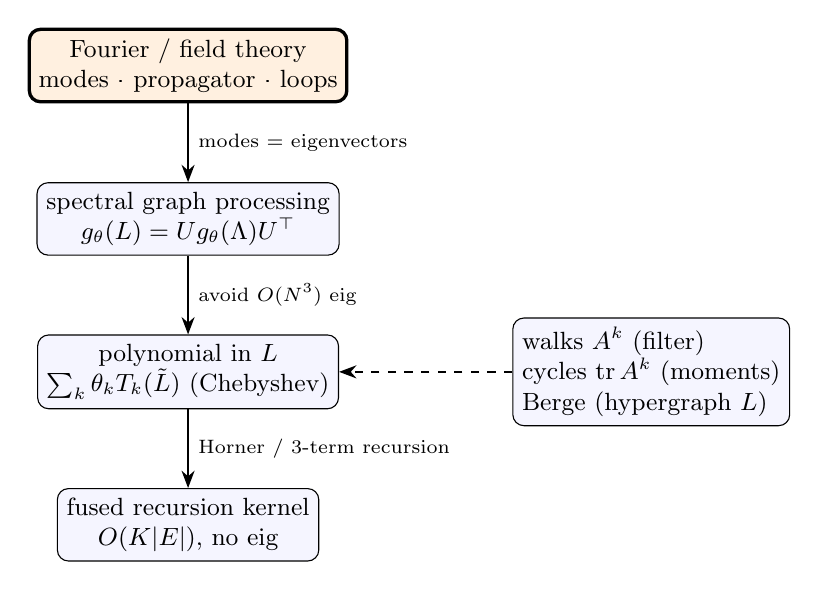
\begin{tikzpicture}[node distance=6mm and 16mm]
  \node[hl] (ft) {Fourier / field theory\\modes · propagator · loops};
  \node[box, below=10mm of ft] (sp) {spectral graph processing\\$g_\theta(L)=U g_\theta(\Lambda)U^\top$};
  \node[box, below=10mm of sp] (poly) {polynomial in $L$\\$\sum_k\theta_k T_k(\tilde L)$  (Chebyshev)};
  \node[box, below=10mm of poly] (ker) {fused recursion kernel\\$O(K|E|)$, no eig};
  \draw[arr] (ft)-- node[right,font=\scriptsize]{modes $=$ eigenvectors} (sp);
  \draw[arr] (sp)-- node[right,font=\scriptsize]{avoid $O(N^3)$ eig} (poly);
  \draw[arr] (poly)-- node[right,font=\scriptsize]{Horner / 3-term recursion} (ker);
  \node[box, right=22mm of poly, align=left] (obj) {walks $A^k$ (filter)\\cycles $\operatorname{tr}A^k$ (moments)\\Berge (hypergraph $L$)};
  \draw[arr, dashed] (obj)-- (poly);
\end{tikzpicture}
\caption{The Fourier/field-theory intent descends to a polynomial in $L$, evaluated by the fused kernel ---
the acceleration is "no eigendecomposition," not magic. Walks/cycles/Berge are the spectral components fed in.}
\end{figure}

\section{Honest ledger + falsifiable tests}
\begin{itemize}[nosep]
  \item \grd{} GFT, ChebNet $O(K|E|)$ filters, heat-kernel/zeta/moment $\leftrightarrow$ walk/cycle
        correspondences --- all established for graphs; the fused kernel accelerates the polynomial evaluation
        (measured: forward at \code{tanh} parity).
  \item \opn{} \textbf{Does a degree-$K$ Chebyshev spectral filter beat $K{=}1$ message passing} on a
        real-topology RL task, params-matched, multi-seed? (The first concrete experiment.)
  \item \opn{} \textbf{Heat-kernel / walk features} $e^{-tL}h$ as a state encoding vs.\ raw node features.
  \item \opn{} \textbf{Signed cycle / zeta features} (the loop expansion) as a structural-entropy signal ---
        ties directly to the entropy-feedback line ($H_{\text{struct}}$ over arity/sign/degree is a spectral
        statistic).
  \item \opn{} The \textbf{signed-hypergraph} spectral theory itself (signed/Berge Laplacian, signed Ihara
        zeta) --- where the novelty, if any, lives.
\end{itemize}
Every one is gated by the same discipline as the rest of the project: a params-matched control and a
$\ge$-parity / $>$-IQR gate before crediting the spectral machinery over plain message passing.

\section{Recommendation}
The fused polynomial kernel is the shared accelerator; the spectral filter is its operator-valued instance.
The cheapest first probe is a \textbf{Chebyshev filter (small $K$) on the signed kinematic hypergraph}, built on
the same kernel, benchmarked and accuracy-gated against $K{=}1$ message passing --- if it lifts a real-topology
task, the ``Fourier field theory'' framing has earned its keep computationally; if not, it remains an elegant
lens and a toolbox (zeta, heat kernel) we can still mine for structural-entropy signals. Either way the claim is
tested, never asserted.
\end{document}
